%%%%%%%%%%%%%%%%%%%%%%%%%%%%%%%%%%%%%%%%%
% Beamer Presentation
% LaTeX Template
% Version 1.0 (10/11/12)
%
% This template has been downloaded from:
% http://www.LaTeXTemplates.com
%
% License:
% CC BY-NC-SA 3.0 (http://creativecommons.org/licenses/by-nc-sa/3.0/)
%
%%%%%%%%%%%%%%%%%%%%%%%%%%%%%%%%%%%%%%%%%

%----------------------------------------------------------------------------------------
%	PACKAGES AND THEMES
%----------------------------------------------------------------------------------------

\documentclass{beamer}

\mode<presentation>{

% The Beamer class comes with a number of default slide themes
% which change the colors and layouts of slides. Below this is a list
% of all the themes, uncomment each in turn to see what they look like.

%\usetheme{default}
%\usetheme{AnnArbor}
%\usetheme{Antibes}
%\usetheme{Bergen}
%\usetheme{Berkeley}
%\usetheme{Berlin}
%\usetheme{Boadilla}
%\usetheme{CambridgeUS}
%\usetheme{Copenhagen}
%\usetheme{Darmstadt}
%\usetheme{Dresden}
%\usetheme{Frankfurt}
%\usetheme{Goettingen}
%\usetheme{Hannover}
%\usetheme{Ilmenau}
%\usetheme{JuanLesPins}
%\usetheme{Luebeck}
%\usetheme{Madrid}
\usetheme[sectionpage=progressbar, numbering=fraction]{metropolis}
%\usetheme{Malmoe}
%\usetheme{Marburg}
%\usetheme{Montpellier}
%\usetheme{PaloAlto}
%\usetheme{Pittsburgh}
%\usetheme{Rochester}
%\usetheme{Singapore}
%\usetheme{Szeged}
%\usetheme{Warsaw}

% As well as themes, the Beamer class has a number of color themes
% for any slide theme. Uncomment each of these in turn to see how it
% changes the colors of your current slide theme.

%\usecolortheme{albatross}
%\usecolortheme{beaver}
%\usecolortheme{beetle}
%\usecolortheme{crane}
%\usecolortheme{dolphin}
%\usecolortheme{dove}
%\usecolortheme{fly}
%\usecolortheme{lily}
%\usecolortheme{orchid}
%\usecolortheme{rose}
%\usecolortheme{seagull}
%\usecolortheme{seahorse}
%\usecolortheme{whale}
%\usecolortheme{wolverine}

%\setbeamertemplate{footline} % To remove the footer line in all slides uncomment this line
%\setbeamertemplate{footline}[page number] % To replace the footer line in all slides with a simple slide count uncomment this line

%\setbeamertemplate{navigation symbols}{} % To remove the navigation symbols from the bottom of all slides uncomment this line

}

% http://www-ljk.imag.fr/membres/Jerome.Lelong/latex/appendixnumberbeamer.sty
% Reference: http://tex.stackexchange.com/questions/2541/beamer-frame-numbering-in-appendix
\usepackage{appendixnumberbeamer}
% Add total frame count to slides, optional. From Stefan,
% http://www.latex-community.org/forum/viewtopic.php?f=4&t=2173
\expandafter\def\expandafter\insertshorttitle\expandafter{%
  \insertshorttitle\hfill\insertframenumber\,/\,\inserttotalframenumber}

\makeatletter
\newcommand{\srcsize}{\@setfontsize{\srcsize}{5pt}{5pt}}
\makeatother

\newcommand{\makesection}{%
  \begin{frame}This is a slide.\end{frame}
  \subsection{First Subsection}
  \begin{frame}This is a slide.\end{frame}
  \subsection{Second Subsection}
  \begin{frame}This is a slide.\end{frame}
}

\usepackage{mathtools}
\usepackage{tabularx}
\usepackage{mdframed}

\usepackage[english]{babel}
\usepackage[utf8]{inputenc}

\newcommand{\backupbegin}{
   \newcounter{finalframe}
   \setcounter{finalframe}{\value{framenumber}}
}
\newcommand{\backupend}{
   \setcounter{framenumber}{\value{finalframe}}
}

\usepackage{soul} % use this (many fancier options)

\usepackage{listings}
\lstset{
  language=JAVA,
  captionpos=b,
  escapeinside={(*@}{@*)}, 
  breaklines=true
}

\newcommand{\rot}[1]{\rotatebox{#1}}
\usepackage{tabularx}

\usepackage{algorithm}
\usepackage{algorithmic}
\renewcommand{\algorithmicrequire}{\textbf{Input:}}
\renewcommand{\algorithmicensure}{\textbf{Output:}}

\newcommand*\rotvertical{\rotatebox{90}}
\newcommand*\rotlarge{\rotatebox{70}}

\newcommand{\Iampl}{\emph{I-Amplification}}
\newcommand{\Aampl}{\emph{A-Amplification}}

\definecolor{ForestGreen}{rgb}{0.13,0.54,0.13}

\usepackage{adjustbox}

\usepackage{graphicx} % Allows including images
\usepackage{booktabs} % Allows the use of \toprule, \midrule and \bottomrule in tables

%----------------------------------------------------------------------------------------
%	TITLE PAGE
%----------------------------------------------------------------------------------------

\title[Test Generation]{Test Generation} % The short title appears at the bottom of every slide, the full title is only on the title page

\author{Benjamin DANGLOT} % Your name
\institute[DIBRIS] % Your institution as it will appear on the bottom of every slide, may be shorthand to save space
{
\medskip
\textit{} % Your email address
}
\date{12th, May 2017} % Date, can be changed to a custom date

\begin{document}
\tracingall


\begin{frame}
\maketitle
\end{frame}

\begin{frame}{Instrumentation and Test Generation}
    \begin{center}
        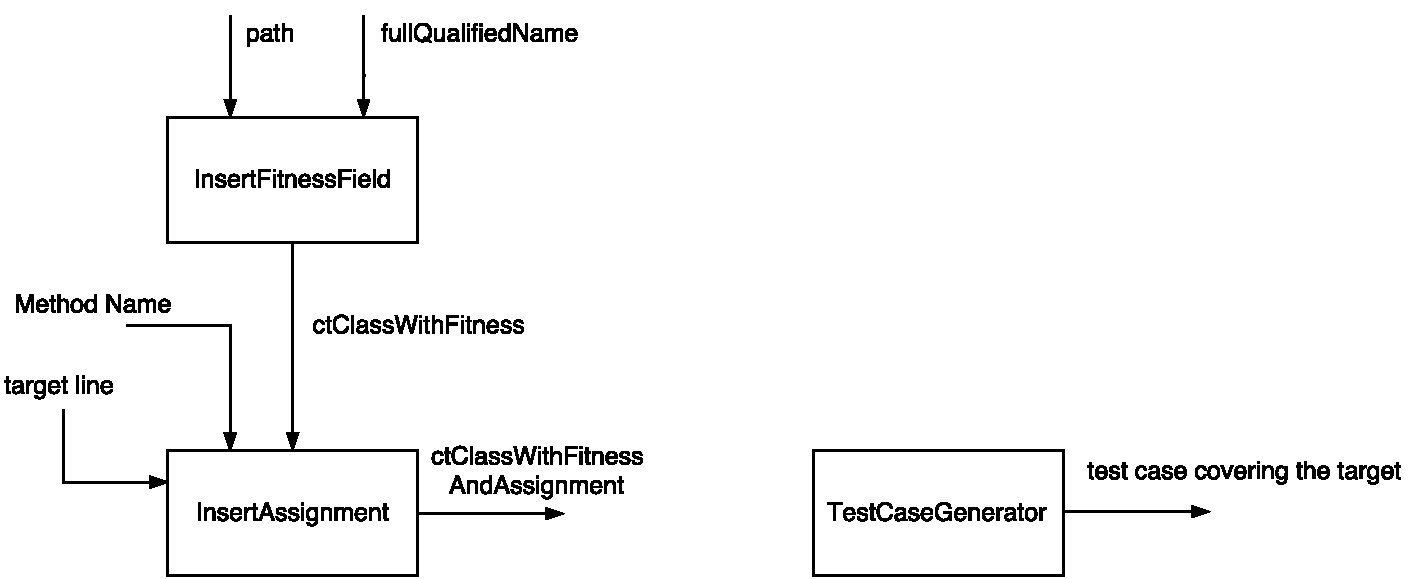
\includegraphics[scale=0.45]{diagram_1.pdf}
    \end{center}
\end{frame}

\begin{frame}{Hill Climbing Algorithm}
3 Algorithms:
    \begin{itemize}
    \item HillClimbing Best: Take the best solution over the neighbors (6 potentials)
    \item HillClimbing First: Take the first solution that improve the fitness
    \item Random: generate new random solution and keep it if it better
    \end{itemize}
Neighbors:
    \begin{itemize}
    \item Random neighbor: replace one value by a random one.
    \item Inc1Neighbors: +1 on one value of the vector solution.
    \end{itemize}
\end{frame}

\begin{frame}{Empirical results: Answer to the RQs}
\begin{center}
\begin{tabular}{ll}
HillClimbing Best Selection: &768 success\\
HillClimbing First Selection: &806 success\\
Random: &254 success\\
\end{tabular}
\begin{mdframed}
\textbf{$RQ_1$}: Yes, the Hill Climbing algorithm is more effective than a Random Algorithm.
\end{mdframed}
\end{center}
\end{frame}

\begin{frame}{Empirical results: Budgets}
\begin{center}
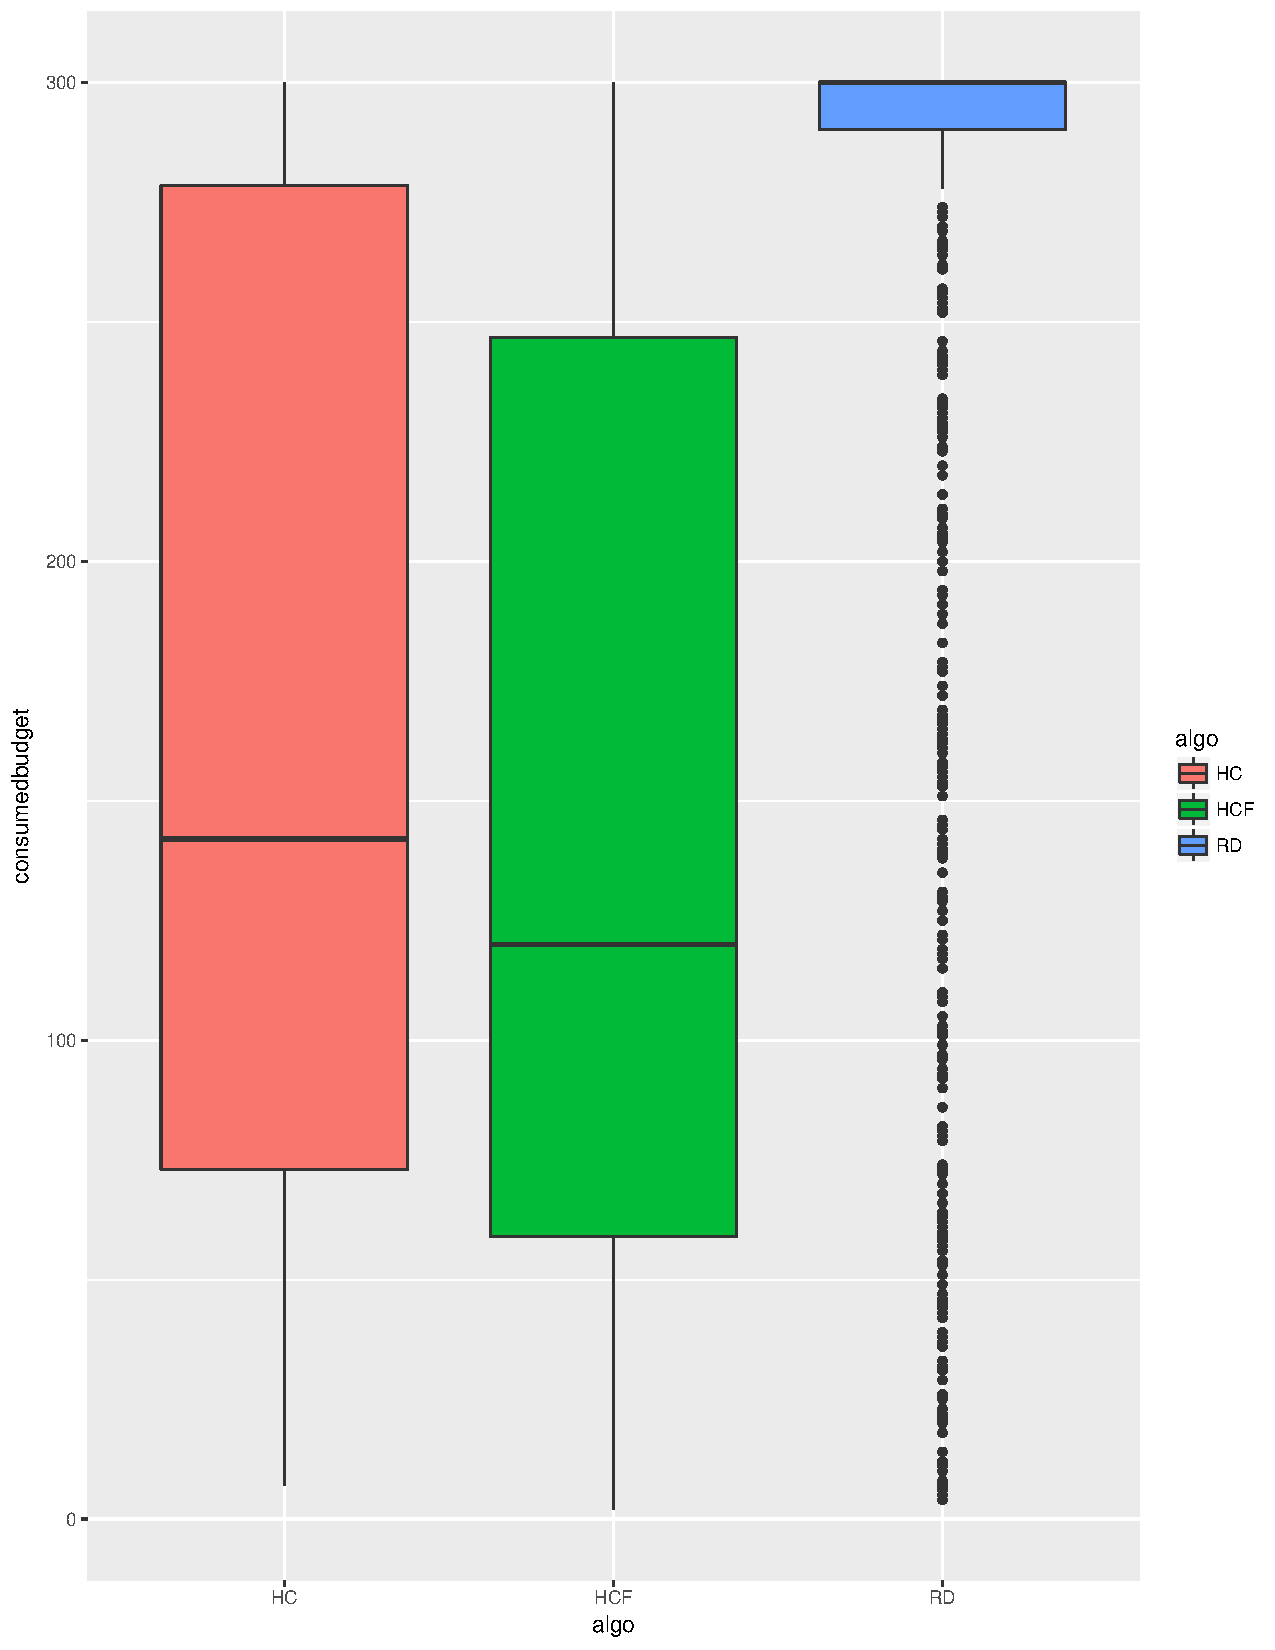
\includegraphics[angle=-90,origin=c,scale=0.2]{boxplot_budgets.pdf}
\begin{mdframed}
\textbf{$RQ_2$}: Yes, the Hill Climbing algorithm is more effecient than a Random Algorithm.
\end{mdframed}
\end{center}
\end{frame}

\begin{frame}{Empirical results: impact of Budgets and Bounds}
\begin{columns}
\begin{column}{0.5\textwidth}
    \begin{center}
        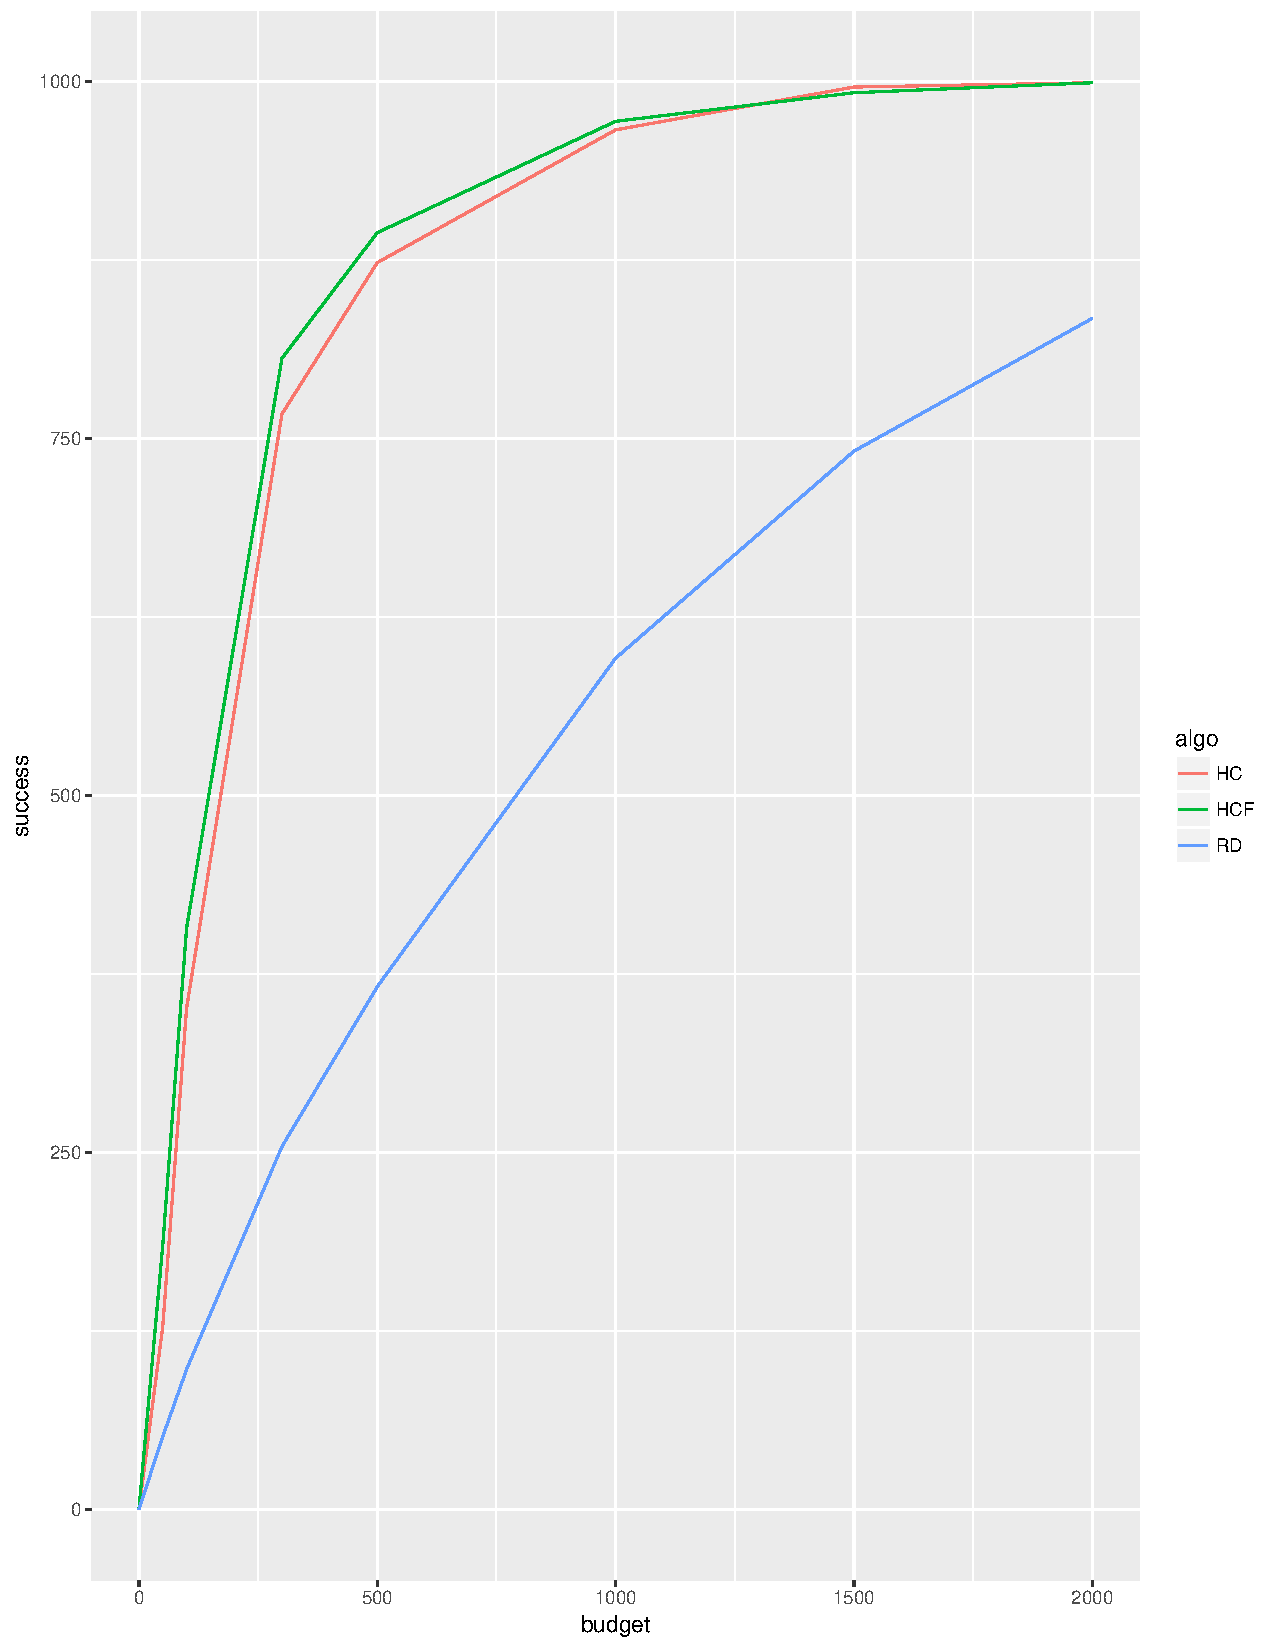
\includegraphics[scale=0.25]{success_f_budget.pdf}
    \end{center}
\end{column}
\begin{column}{0.5\textwidth}
    \begin{center}
        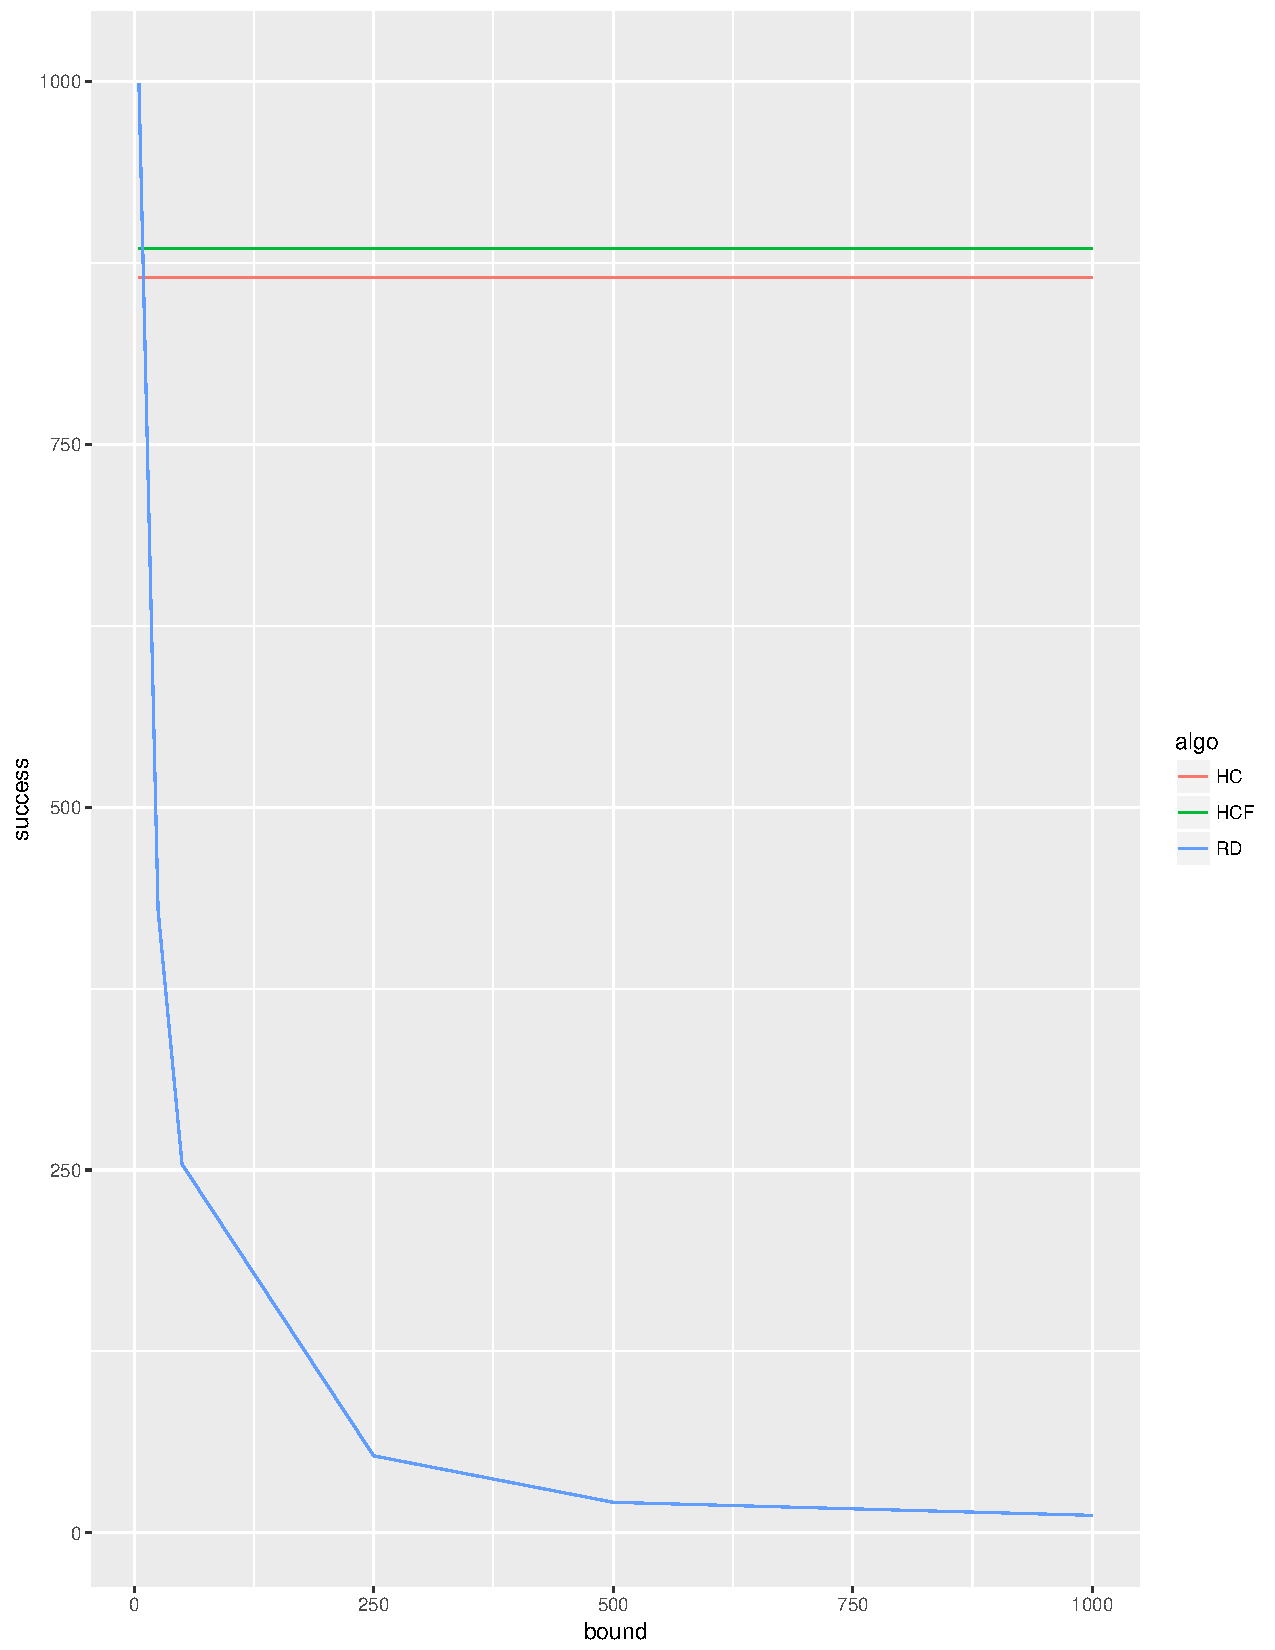
\includegraphics[scale=0.25]{success_f_bound.pdf}
    \end{center}
\end{column}
\end{columns}
\end{frame}

\begin{frame}{Statistical Analysis}

\begin{columns}
\begin{column}{0.5\textwidth}
Fisher test result on the number of success:
\begin{mdframed}
\begin{itemize}
\item p-value $< 2.2e-16$
\item alternative hypothesis: true odds ratio is not equal to 1
\item 95 percent confidence interval: 7.798722 11.856348
\end{itemize}
\end{mdframed}
\end{column}
\begin{column}{0.5\textwidth}
Wilcoxon test on the consumed budged:
\begin{mdframed}
\begin{itemize}
\item W = 234970, p-value < 2.2e-16
\item alternative hypothesis: true location shift is not equal to 0
\end{itemize}
\end{mdframed}
\end{column}
\end{columns}
\end{frame}


\begin{frame}{Possible Improvement}
Run the Test Generator over multiple target:
\begin{itemize}
\item Add a loop over all target
\item Instrument the class according to the current target
\item Add the compilation of the instrumented class by Spoon
\item Build a custom $ClassLoader$ with the previous compiled file
\item Run the HillClimbing to generate test case for the current target (using reflection)
\item Generate the test cases with Spoon
\end{itemize}
\end{frame}

\begin{frame}{About Me}

\includegraphics[scale=0.25]{logo_readme_md.png}\\
From Lille, France. Phd Student at Inria.\\
Within H2020 STAMP: \textbf{S}oftware \textbf{T}esting \textbf{AMP}lification.\\
\center
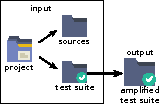
\includegraphics[scale=2]{dspot_1.pdf}
\end{frame}

\begin{frame}{DSpot}
\begin{center}
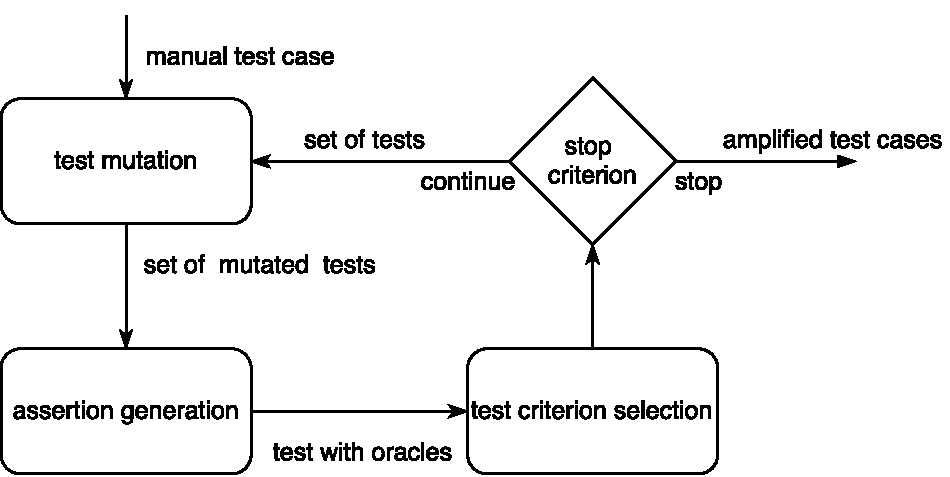
\includegraphics[scale=0.6]{workflow.pdf}
\end{center}
\end{frame}

\end{document}
